\documentclass[12pt,a4paper]{report}

\usepackage[spanish]{babel}
\usepackage[T1]{fontenc}
\usepackage[utf8]{inputenc}
\usepackage{amsmath}
\usepackage{graphicx}
\usepackage[page]{appendix}
\usepackage{listings}
\usepackage{color}
\usepackage{float}
\usepackage{rotating}
\usepackage{graphicx}
\newcommand\scalemath[2]{\scalebox{#1}{\mbox{\ensuremath{\displaystyle #2}}}}

\addto\captionsspanish{\renewcommand\appendixpagename{Archivos de código}}

\DeclareFixedFont{\ttb}{T1}{txtt}{bx}{n}{9}
\DeclareFixedFont{\ttm}{T1}{txtt}{m}{n}{9} 
\DeclareFixedFont{\tti}{T1}{txtt}{m}{it}{9}
\definecolor{comment}{RGB}{150,150,150}

\lstset{
	frame = single, 
	extendedchars=true,	
	showstringspaces=false,
	inputencoding=latin1,
	literate={á}{{\'a}}1 {é}{{\'e}}1 {í}{{\'i}}1 {ó}{{\'o}}1 {ú}{{\'u}}1 {ñ}{{\~n}}1
	{Á}{{\'A}}1 {É}{{\'E}}1 {Í}{{\'I}}1 {Ó}{{\'O}}1 {Ú}{{\'U}}1,
	language=Python,
	basicstyle=\ttm,
	otherkeywords={self},
	keywordstyle=\ttb,
	commentstyle=\tti\color{comment}
	}




% Indica el título del documento como la palabra "Práctica " seguida del número de práctica.
\title{Práctica 3}

% Indica tu nombre completo
\author{Antonio Jesús Heredia Castillo}

\begin{document}

\maketitle

\section*{Ejercicio 1}
Para implementar la función tenemos que hacer uso de las deducciones que se realizan en la memoria.\\
\\
 Aunque tenemos algunos coeficientes que le pongo directamente el valor a 0, esto se debe a que como sabemos que la aceleración y velocidad al inicio y al final son nulos. Estos coeficientes con valor a 0 son $c_{12}$, $c_{11}$,$c_{32}$ y $c_{31}$. Otros coeficientes tendrán el valor de las articulaciones, estos son $c_{10}=qI$, $c_{20}=qD$ y $c_{30}=qF$.\\
 \\
 La matriz que tenemos que obtener su inverso tendrá el valor de:
 $$M=\left[\begin{array}{ccccccc}
 1 & 1 & 0 & 0 & 0 & 0 & 0 \\
 \frac{3}{t_{1}} & \frac{4}{t_{1}} & -\frac{1}{t_{2}} & 0 & 0 & 0 & 0 \\
 \frac{6}{t_{1}^{2}} & \frac{12}{t_{1}^{2}} & 0 & -\frac{2}{t_{2}^{2}} & 0 & 0 & 0 \\
 0 & 0 & 1 & 1 & 1 & 0 & 0 \\
 0 & 0 & 0 & 0 & 0 & -1 & 1 \\
 0 & 0 & \frac{1}{t_{2}} & \frac{2}{t_{2}} & \frac{3}{t_{2}} & -\frac{3}{t_{3}} & \frac{4}{t_{3}} \\
 0 & 0 & 0 & \frac{2}{t_{2}^{2}} & \frac{6}{t_{2}^{2}} & \frac{6}{t_{3}^{2}} & -\frac{12}{t_{3}^{2}}
 \end{array}\right]^{-1}$$
 Y la matriz columna:
 $$V=\left[\begin{array}{c}
 qD-qI\\
 0\\
 0 \\
 qA-qD \\
 qA-qF\\
 0\\
 0
 \end{array}\right]$$
 Como podemos ver he quitado algunos valores de la matriz columna original. Esto se debe a que debido a la aceleración y velocidad igual a 0, desaparecían.\\
 \\
 Solo tendremos que multiplicar $M\times V$. Y los valores de los coeficientes que nos faltaban por obtener los tendremos ahí.
 \section*{Ejercicio 2}
 Gracias a lo realizado en practicas anteriores podemos realizar este ejercicio rápidamente. Realizaremos los siguientes pasos:
 \begin{enumerate}
 	\item Tenemos que hacer es uso de la cinemática inversa para conseguir el valor de ambas articulaciones en los puntos intermedios.
 	\item Obtendremos los coeficientes de ambas articulaciones en la trayectoria 4-3-4 haciendo uso de la función implementada en el ejercicio anterior.
 	\item Evaluaremos los tres polinomios (uno por cada segmento) de las dos articulaciones en el rango que nos indica el guión de practicas. Cada ``tramo'' tendrá un tiempo de un segundo y avanzaremos de $0.05$.
 	\item Por ultimo concatenamos los tres segmentos que recorre cada articulación y podremos ver el recorrido de la trayectoria.
 	\item Para ver el recorrido de la trayectoria usaremos funciones implementadas en practicas anteriores.
\end{enumerate}	
Como resultado tendremos:
\begin{figure}[H]
	\centering
	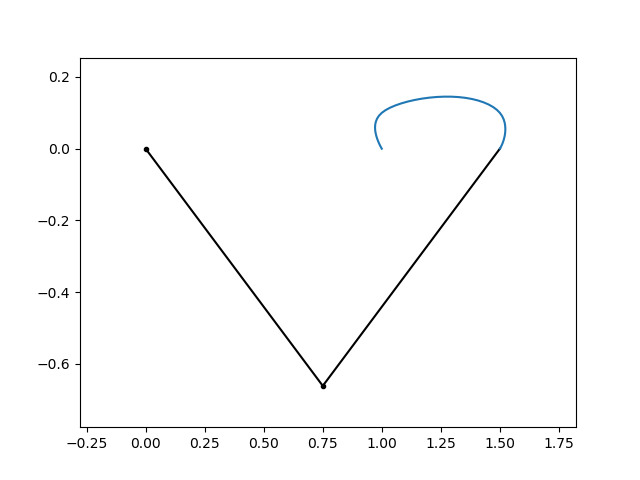
\includegraphics[width=0.7\linewidth]{img/anima.png}
	\caption{Trayectoria realizada}
	\label{fig:ej4}
\end{figure}
Supongo que el brazo de mi robot aparece del revés debido a que tendré algún símbolo cambiado en algún lado. Pero no he sido capaz de encontrar donde.
\begin{appendices}
	\section*{ejercicio1-2.py}
	\lstinputlisting{../codigo.py}


\end{appendices}

\end{document}
